\documentclass[pageno]{jpaper}

%replace XXX with the submission number you are given from the ASPLOS submission site.
\newcommand{\asplossubmissionnumber}{XXX}

\usepackage[normalem]{ulem}
\usepackage{listings}
\usepackage{graphicx}

\begin{document}

\title{A Static Analysis Approach for Supporting Concurrency in Partitioned Program}

\date{}
\maketitle
\thispagestyle{empty}

\begin{abstract} 
  Program partitioning is an effective way to improve program security. However, there are still many limitations that prevent partitioning framework from being deployed on the vat majority of modern high-performance programs. In this paper, we identify two key limitations. First, existing partitioning frameworks cannot support concurrent systems due to potential incorrect data synchronization problem. Second, most of partitioning framework normally synchronize more data than necessary, which decrease communication efficiency among partitions and thus cause lower performance. To address these two limitations, we provide two techniques to assist existing partitioning frameworks to support concurrency and avoid synchronizing unneeded data across partition boundary. We implemented our techniques on top of LXDs partitioning framework and evaluate them on a set of Linux drivers. The experiments results shows that our techniques can help existing programs to ...
\end{abstract}

\section{Introduction}
Program partitioning refers to the process of separating an existing program into multiple partitions. Each partition runs in a separated domain has its own set of data and privileges. Data are synchronized among different domains through remote procedure call mechanisms. This approach improves program security because compromising one partition doesn't lead to the compromise of other partitions. For programs written in low-level, type-unsafe languages such as C and C++, the partitioning technique is especially beneficial for security as these programs are prone to attack.

There are many attempts on enforcing kernel isolation in recent years. For example, Microdriver... try to isolated drivers from kernel and run the drivers in separate domain. 

However, existing kernel isolation frameworks are hard to be deployed correctly on nowadays high-performance operating systems due to many limitations. In this work, we made our observation based on the experiments of previous isolation mechanisms and identify two critical limitations. 

First, existing isolation mechanisms do not consider concurrency in their design. In a common isolation architecture, domains synchronize data in a sender-and-receiver analogy: a sender thread and a receiver thread communicate with each other in a serial manner and data synchronization in done synchronously. However, in concurrent programs, asynchronous accesses to data is allowed and thus there is a window of time during which a domain may execute on incorrect data. 

Second, most of mechanisms synchronize more data than necessary across partition boundary. When passing large data structure across partition boundaries, a common synchronization strategy is marshalling/unmarshalling all data structure fields. This greedy approach may incur significant communication overhead when domain transition is frequent in a program. In addition, passing all fields across domain also harms security as high-privileged and sensitive fields within data structures may also be synchronized to low-privileged partitions.

We argue that these two problems need to be addressed in existing isolation mechanisms as they are critical to isolation mechanisms runtime efficiency and correctness. 

In this paper, we implemented a tool called SADS, which provides two static analyses to address the two problems we described above. The analyses are implemented in the LXDs kernel isolation framework. We consider our major contribution as follows:

\begin{enumerate}
  \item Provide a tool called SADS which provides two important static analyses to address data synchronization problems in current kernel isolation frameworks.
  \item Analysis 1: computes data that need to be synchronized across domain boundaries during domain communication time. The core of the technique is a static analysis which computes data structure fields that being accessed for each cross-domain function call. One important feature that distinguishes this static analysis from previous works is that it consider domain privacy and prevent synchronizing domain private data at communication time. The key component to allow this is another static analysis for computing domain shared data, which we will describe in details in Section. .
  \item Analysis 2: addresses potential data synchronization problems for concurrent programs. In concurrent partitioning programs, data accesses can modified in asynchronous context. This creates potential incorrect data synchronization problem. We illustrate this problem in Section. To address this problem, we provide another static analysis that can identify possible program locations where data synchronization problem can occur and also computes the data that need to be correctly synchronized.
\end{enumerate}

The SADS tool is implemented inside LLVM and integrated with the LXDs kernel partitioning framework. We evaluate the correctness and efficiency of SADS on a set of Linux drivers. The results suggests that SADS can be integrated in practical kernel isolation mechanisms to address potential data synchronization problems.

\section{Background and Related Work}
In our knowledge, no existing partitioning frameworks have addressed these two problems together. 

\paragraph{Program Partitioning} PtrSplit is an automatic partitioning system aims that provide mashalling/unmarshalling of pointer type data. The system is capable of generating code that performs marshalling and unmarshalling. While PtrSplit can be applied on many single-threaded program, it fail to address concurrent programs. In addition, the generated communication code by PtrSplit marshalling all fields in data structures that are passed across domain. Thus, none of the two problems are addressed by this system.

\paragraph{Kernel Isolation} The Microdriver system \cite{ganapathy2008design} provides an architecture for partitioning driver from kernel and allow developers to develop user-mode driver based on it. In this work, a component called code generator is used to generate marshaling/unmarshaling code for data structures passed across partition boundary. This component relies on a static analysis called field accessed analysis, which computes a set of fields that need to be synchronized across domain. Thus, the amount of data structure data passed across boundaries are largely reduced. However, the component has two critical limitations. First, the analysis doesn't consider high-privilege data fields that are private to certain partitions. This indicates that some sensitive data can be synchronized to low-privileged partition. Second, the analysis doesn't describe the computation of fields that may get accessed in concurrent context. Thus, we consider this analysis only partially address the second problem. 

\section{System Overview}
The SADS system provides two core components to address the data synchronization problems in concurrent partitioning program. As the two components are designed and implemented in the form of LLVM pass, SADS can be incorporated into existing partitioning frameworks. Figure.\ref{figs:system_workflow} shows the overall workflow of SADS. The system first takes the source code of the target program and convert them to LLVM IR using LLVM's frontend. Afterwards, SDAS build a Program Dependency Graph (PDG) using the LLVM IR. Next, two components use the PDG to compute necessary for addressing the data synchronization problems. 

The first component is used to improve data communication efficiency among partitions. The component computes a set of necessary fields that need to be passed across partition boundary during inter-domain communications. These data is organized in the form of projection, which is a mechanism for describing data structure fields that need to be synchronized. 

The second component addresses potential data synchronization problem for concurrent programs. The component also uses PDG to reason about program locations where data synchronization problems may occur. 

The fundamental components for the two static analyses is a Program Dependency Graph (PDG), which represents the data and control dependencies in the whole program. Based on the PDG, the first component "compute projection" computes data structure fields that need to be synchronized across separation boundary.

\begin{figure}[th]
  \centering
  \includegraphics[width=0.9\linewidth]{figs/system_overview.png}
  \caption{The workflow of SADS toolchain.}
  \label{figs:system_workflow}
\end{figure}    


\section{Design}
\subsection{PDG Construction}
Our analysis for automatic IDL generation is based on the
\textit{Program Dependence Graph (PDG)}~\cite{Ferrante87PDG}
representation of a program. Conceptually a PDG represents
a program's control and data dependence in a single graph.
Our PDG construction builds on top of
PtrSplit~\cite{LiuTJ17Ptrsplit} and extends it with field sensitivity,
which is necessary for computing projections.  Next we provide a brief
overview of our PDG construction; details of PDG construction other
than field sensitivity can be found in PtrSplit.

Our analysis builds a PDG for an LLVM IR program. In the intraprocedual
portion of the PDG, nodes represent IR instructions and edges represent
various kinds of control and data dependencies within functions.  One
example kind is read-after-write data dependence: if instruction
n1 reads a piece of memory that was written by n2, there is a data
dependence edge from n2 to n1 and the edge is attached with a label
that denotes the piece of memory in question.

The interprocedural portion of a PDG adopts an approach called
\textit{parameter trees}, a type-based representation that enables
modular interprocedural PDG construction. The parameter tree for a
parameter is a tree representation of all possible
storage locations that a function can access through the parameter. 
%
In the example below a struct pointer is passed to function \textit{foo} and the
struct has two fields.
\begin{lstlisting}[label=lst:hierarchies] 
struct st {int a, float b};
void foo (struct st* s) {...}
\end{lstlisting}

\begin{figure}[t]
   \centering
   \includegraphics[width=0.4\columnwidth]{figs/parameter_tree_example-a}
	\caption{Parameter tree for foo()'s parameter s.}
   \label{fig:parameter_tree}
\end{figure}

The parameter tree for the parameter {\tt s} is shown in
\autoref{fig:parameter_tree}. Each node in the parameter tree
represents storage that {\tt foo} can access through {\tt
  s}. Therefore, the tree has a node for the pointer to the struct, a
node for the struct, and one node for each of the two
fields. Parameter trees enable modular interprocedural PDG
construction without requiring a global alias analysis, through
building actual parameter trees for arguments at a call site and
formal parameter trees for parameters of functions (and adding
necessary edges); details can be found in~\cite{LiuTJ17Ptrsplit}.

%% Parameter trees enable modular interprocedural construction in the
%% following way.  A formal parameter tree is constructed for each
%% parameter of a function.  At a function call site, an actual parameter
%% tree is constructed for each argument.  Further data-dependence edges
%% are added between nodes in an actual tree with corresponding nodes in
%% a formal tree to represent interprocedual dataflow. Finally, in each
%% function, data-dependence edges are added from parameter tree nodes to
%% instruction nodes that access the nodes' corresponding storage;
%% similar edges are added in a caller for nodes in an actual tree.

%% When adding data dependency edges from parameter tree to
%% intra-function instruction nodes, we also consider alias
%% information.

Our static analysis extends the parameter-tree based PDG construction
of PtrSplit with field sensitivity. In particular, when an instruction
accesses a particular field of a struct parameter, a data-dependence
edge is added between the instruction and the node that represents the
field in the parameter tree. In contrast, being field insensitive,
PtrSplit adds edges between the instruction and all field nodes in the
parameter tree. Field sensitivity is essential for computing
projections, which requires an understanding of what fields are
read/written by the callee domain when a struct is passed.  Our
implementation of field sensitivity takes advantage of the fact that,
in the LLVM IR, the {\tt GetElementPtr} (GEP) instruction is
used to compute the offset of a field; by tracking what offsets are
computed by GEP instructions, our analysis resolves the targets of 
struct reads/writes for most of the cases.

\subsection{Identify Cross-domain Function Invocations}
The following steps are used to compute a set of cross-domain function calls for each partition:
\begin{enumerate}
  \item Identify undefined functions in a partition through LLVM.
  \item Create a list of library calls.
  \item For each undefined function which is not in the list of library calls, we consider it as a cross-domain function call.
\end{enumerate}

On important problem to consider in these steps is finding indirect called functions. For each indirect call, we use the sea-dsa pointer analysis to find out possibly called indirect functions for each indirect call.

\subsection{Compute Shared Data}
A data is considered shared between two partitions if it has accesses in both of them. The set of shared data specifies what is allowed to be exchanged between two partitions. The role of shared data is essential in both techniques. In projection computation, shared data is used to prevent private data from being synchronized to other partitions. In the process of computing data that need to be synchronized at the end of atomic regions, we only generate summary for shared data.

In general, we use a type-based approach to compute shared data between two partitions. One greedy approach to compute shared data is considering all types of data appear in the program as shared and then computes how this data is accessed. However, this approach is inefficient as it's likely that only a small subset of data types are actually shared. Thus, we first computes a subset of data types that are shared between two domains, and then computes how the variables of these data types are accessed. 

We compute shared data types starting from the possible communication channels between two partitions. In a common partitioned program, two partitions can communicate through two channels: 1. global variables and 2. cross-domain functions. Thus, we consider the data types used in these two channels as possible shared data type. Next, we can further optimize the computation of shared data types by excluding global variables that has uses in only one partition (module). The above steps compute a set of shared data types between two partitions. 

After obtaining shared data types, the next step is computing actually shared data. For non-struct types, we simply consider the data is shared between the two domains. For data structure types, we use a global map to store the access information for them; the map key is a data structure type and the value is a set of fields accessed through the type. 

The global map is computed through \textbf{global type tree}. The algorithm of constructing global type tree is the same as the algorithm of constructing parameter tree. The different is that each global type tree node represents a data field in a data structure type. We mark a node as visited if the corresponding field is accessed in the program.

To compute the accesses to each data field, we add dependency edges between the global tree nodes and variable of the same type. The detailed . steps are as follow: We first find a set of IR variables \textbf{TV} that match the root node's type in the program and add a \textbf{TYPE\_MATCH} dependency edge between the root node and the variables. Next, we compute TV for the rest of tree node using PDG: for each tree node \textbf{n}, we iterate through the user (IR variables) of its parent node’s TV and find those having the same type and offset with the child node. These variables are included in n's TV. Then, we add TYPE MATCH dependency edge between a child node and the variable nodes in TV. This algorithm is guarantee to terminates since there is not backward edges in global type trees. 

\subsection{Projections}


\paragraph{Compute Projections}
A field is put into projection if it meets any of the following two conditions:

\begin{enumerate}
  \item A field is accessed in the transitive closure of a cross-domain function invocation.
  \item A field is accessed in asynchronous call context.
\end{enumerate}

The first condition indicates a field is accessed after being passed across domain. Thus, its state is synchronized according to its access type (read/write). The second condition consider possible accesses to shared data in concurrent programs. The high-level steps for computing the projects are as follows:
\begin{enumerate}
  \item For eah 
\end{enumerate}


\paragraph{Optimize Projection Through Shared Data}


\subsection{Compute Data Need to be Synchronized in Atomic Region}
\paragraph{Compute Atomic Region}


\section{Implementation}

\subsection{}


\section{Evaluation}


\section{Conclusion}


\section{Acknowledgement}



The submission instructions are also available in this
\href{https://asplos-conference.org/submissions/}{this website},
including a link to the paper submission site. The website contains
sample PDF files for the
\href{https://asplos-conference.org/wp-content/uploads/2020/06/asplos21-paper-template.pdf}{paper} and
\href{https://asplos-conference.org/wp-content/uploads/2020/06/asplos21-extended-abstract-template.pdf}{extended abstract}. The
sample files are formatted using the ASPLOS'21 submission format and
contain the submission and formatting guidelines. The website also
includes an \href{https://asplos-conference.org/wp-content/uploads/2020/06/asplos21-templates.zip}{archive file}
with \LaTeX~templates for both papers and extended abstracts.

All questions regarding paper formatting and submission should be directed
to the program co-chairs.

\paragraph{Important highlights:}
\begin{itemize}
\item Papers should contain a
maximum of 10 pages of single-spaced two-column text, including any
appendixes, but not including references.
\item All submitted papers must be accompanied by an extended
  abstract, in a separate file with a maximum of 
2 pages of single-spaced two-column text, not including references.
\item Papers and extended abstracts must be submitted in printable PDF format.
\item Text must be in a minimum 10pt ({\bf not} 9pt) font.
\item No page limit for references for papers and the extended abstracts.
\item Each reference must specify {\em all} authors (no {\em et al.}).
\item Authors of {\em all} accepted papers will be required
  to record a short (less than 2 minute) video that previews the paper.
  This video substitutes for a lightning talk.
  Additional requirements for the video will be forthcoming.
\item Authors of {\em all} accepted papers will be required to have a poster in addition to the regular
conference talk.
\item Proceedings will appear in the ACM digital library up to two weeks
before the conference.
\end{itemize}

\paragraph{Paper evaluation objectives:}
The committee will make every effort to fairly judge each submitted paper on
its own merits. There will be no target acceptance rate.  We expect to
accept a wide range of papers with appropriate expectations for
evaluation. Papers that build on significant past work with
strong evaluations are valuable,  We encourage you to consider the
\href{https://www.sigplan.org/Resources/EmpiricalEvaluation/}{SIGPLAN
  empirical evaluation guidelines} for the evaluation of the ideas in
your paper. At the same time,  papers that open new areas with less
rigorous evaluation are equally welcome and especially encouraged.
Given the wide range of topics covered by ASPLOS, every effort will be
made to find expert reviewers.

This year, ASPLOS will pilot the use of extended abstracts. {\bf All
  papers submissions must be accompanied by a 2-page extended
  abstract, submitted as a separate PDF file}.  Extended abstracts
will be used throughout the reviewing process so that a larger number
of PC members have a better understanding of each paper as they made
decisions.

ASPLOS'21 will also feature Artifact Evaluation for accepted papers. 
Although encouraged, Artifact Evaluation submission is not required nor will 
it be used as a condition for paper acceptance into ASPLOS 2021. Reviewers will 
not have visibility into the availability of such artifacts. We request that 
authors do not refer to them in their paper submissions.

\section{Paper and Abstract Preparation Instructions}

Formatting instructions and \LaTeX~ templates for the paper and
extended abstract can be found on
\href{https://asplos-conference.org/submissions/}{this website}.

\subsection{Paper Formatting}

Papers must be submitted in printable PDF format and should contain a
{\bf maximum of 10 pages} of single-spaced two-column text, including any
appendixes, but {\bf not
  including references}.  You may include any number of pages for
references, but see below for more instructions.  If you are using
\LaTeX~\cite{lamport94} to typeset your paper, then we suggest that
you use \href{https://asplos-conference.org/wp-content/uploads/2020/06/asplos21-templates.zip}{this template}.
If you use a different
software package to typeset your paper, then please adhere to the
guidelines given in Table~\ref{table:formatting}.

\begin{table}[h!]
  \centering
  \begin{tabular}{|l|l|}
    \hline
    \textbf{Field} & \textbf{Value}\\
    \hline
    \hline
    File format & PDF \\
    \hline
    Page limit & 11 pages, {\bf not including}\\
               & {\bf references}\\
    \hline
    Paper size & US Letter 8.5in $\times$ 11in\\
    \hline
    Top margin & 1in\\
    \hline
    Bottom margin & 1in\\
    \hline
    Left margin & 0.75in\\
    \hline
    Right margin & 0.75in\\
    \hline
    Body & 2-column, single-spaced\\
    \hline
    Separation between columns & 0.25in\\
    \hline
    Body font & 10pt\\
    \hline
    Abstract font & 10pt, italicized\\
    \hline
    Section heading font & 12pt, bold\\
    \hline
    Subsection heading font & 10pt, bold\\
    \hline
    Caption font & 9pt, bold\\
    \hline
    References & 8pt, no page limit, list \\
               & all authors' names\\
    \hline
  \end{tabular}
  \caption{Formatting guidelines for submission. }
  \label{table:formatting}
\end{table}

\textbf{Please ensure that you include page numbers with your
submission}. This makes it easier for the reviewers to refer to different
parts of your paper when they provide comments.

Please ensure that your submission has a banner at the top of the title
page, as shown in
\href{https://asplos-conference.org/wp-content/uploads/2020/06/asplos21-paper-template.pdf}{this
sample paper}, which contains the submission number and the notice of
confidentiality.  If using the template, just replace XXX with your
submission number.

\subsection{Extended Abstract Formatting}

The extended abstracts must be submitted in printable PDF format and should contain a
{\bf maximum of 2 pages} of single-spaced two-column text, {\bf not
  including references}.  You may include any number of pages for
references, but see below for more instructions. The extended
abstracts should use the same formatting as the papers (see \href{https://asplos-conference.org/wp-content/uploads/2020/06/asplos21-paper-template.pdf}{the
paper formatting instructions}. If you are using
\LaTeX~\cite{lamport94} to typeset your extended abstract, then we suggest that
you use
\href{https://asplos-conference.org/wp-content/uploads/2020/06/asplos21-templates.zip}{this
  template} that also describes that information to include in your
extended abstract. 

\subsection{Content}

\noindent\textbf{Author List.}  Reviewing will be \textbf{double blind};
therefore, please \textbf{do not include any author names on any submitted
documents except in the space provided on the submission form}.  You must
also ensure that the metadata included in the PDF does not give away the
authors. If you are improving upon your prior work, refer to your prior
work in the third person and include a full citation for the work in the
bibliography.  For example, if you are building on {\em your own} prior
work in the papers \cite{nicepaper1,nicepaper2,nicepaper3}, you would say
something like: "While the authors of
\cite{nicepaper1,nicepaper2,nicepaper3} did X, Y, and Z, this paper
additionally does W, and is therefore much better."  Do NOT omit or
anonymize references for blind review. There is one exception to this for
your own prior work that appeared in IEEE CAL, workshops without archived
proceedings, etc.\, as discussed later in this document.

\noindent\textbf{Figures and Tables.} Ensure that the figures and tables
are legible.  Please also ensure that you refer to your figures in the main
text.  Many reviewers print the papers in gray-scale. Therefore, if you use
colors for your figures, ensure that the different colors are highly
distinguishable in gray-scale.

\noindent\textbf{References.}  There is no length limit for references.
{\bf Each reference must explicitly list all authors of the paper.  Papers
not meeting this requirement will be rejected.} Authors of NSF proposals
should be familiar with this requirement. Knowing all authors of related
work will help find the best reviewers. Since there is no length limit
for the number of pages used for references, there is no need to save space
here.

\section{Paper and Abstract Submission Instructions}

\subsection{Declaring Authors}

Declare all the authors of the paper up front. Addition/removal of authors
once the paper is accepted will have to be approved by the program co-chairs,
since it potentially undermines the goal of eliminating conflicts for
reviewer assignment.

\subsection{Areas and Topics}

ASPLOS emphasizes multidisciplinary research. Submissions should ideally
emphasize synergy of two or more ASPLOS areas: architecture, programming
languages, operating systems, and related areas (broadly
interpreted). Authors should indicate these areas on the submission form as
well as specific topics covered by the paper for optimal reviewer match. If
you are unsure whether your paper falls within the scope of ASPLOS, please
check with the program co-chair -- ASPLOS is a broad, multidisciplinary
conference and encourages new topics.

\subsection{Declaring Conflicts of Interest}

Authors must register all their conflicts on the paper submission site.
Conflicts are needed to ensure appropriate assignment of reviewers.
If a paper is found to have an undeclared conflict that causes
a problem OR if a paper is found to declare false conflicts in order to
abuse or ``game'' the review system, the paper may be rejected.

Please declare a conflict of interest (COI) with the following people
for any author of your paper:

\begin{enumerate}
\item Your Ph.D. advisor(s), post-doctoral advisor(s), Ph.D. students,
      and post-doctoral advisees, forever.
\item Family relations by blood or marriage and close friends, forever (if they might be potential reviewers). You are a close friend with someone if you have or would spend a night at their home if you were visiting them, or vice versa.
\item People with whom you have collaborated in the last four years, including
\begin{itemize}
\item co-authors of accepted/rejected/pending papers.
\item co-PIs on accepted/rejected/pending grant proposals.
\item funders (decision-makers) of your research grants, and researchers
      whom you fund.
\end{itemize}
\item People (including students) who shared your primary institution(s) in the
last four years.
\end{enumerate}

``Service'' collaborations such as co-authoring a report for a professional
organization, serving on a program committee, or co-presenting
tutorials, do not themselves create a conflict of interest.
Co-authoring a paper that is a compendium of various projects with
no true collaboration among the projects does not constitute a
conflict among the authors of the different projects.

On the other hand, there may be others not covered by the above with whom
you believe a COI exists, for example, close personal friends.
Please report such COIs; however, you may be asked to justify them.
Please be reasonable.	For example, you cannot declare a COI with a
reviewer just because that reviewer works on topics similar to or
related to those in your paper.
The program co-chairs may contact co-authors to explain a COI whose origin is unclear.

We hope to draw most reviewers from the PC and the ERC, but others from the
community may also write reviews.  Please declare all your conflicts (not
just restricted to the PC and ERC).  When in doubt, contact the program
co-chairs.

\subsection{Concurrent Submissions and Workshops}

By submitting a manuscript to ASPLOS'21, the authors guarantee that the
manuscript has not been previously published or accepted for publication in
a substantially similar form in any conference, journal, or workshop. The
only exceptions are (1) workshops without archived proceedings such as in
the ACM digital library (or where the authors chose not to have their paper
appear in the archived proceedings), or (2) venues, such as IEEE CAL, where
there is an explicit policy that such publication does not preclude longer
conference submissions. These are not considered prior publications. 
Technical reports and papers posted on public social media sites, Web pages,
or online repositories, such as arxiv.org, are not considered prior
publications either. In these cases, the submitted manuscript may
ignore the posted work to preserve author anonymity. 
The authors also guarantee that no paper that contains
significant overlap with the contributions of the submitted paper will be
under review for any other conference, journal, or workshop during the
ASPLOS'21 review period. Violation of any of these conditions will lead to
rejection.  As always, if you are in doubt, it is best to contact the
program co-chairs.  Finally, we also note that the ACM Plagiarism Policy
(http://www.acm.org/publications/policies/plagiarism\_policy) covers a range
of ethical issues concerning the misrepresentation of other works or one's
own work.

\subsection{Ethical Obligations}
\begin{itemize}
\item Authors are not allowed to contact reviewers or PC members to encourage or solicit them to bid on any paper.
\item Authors are not allowed to attempt to sway a reviewer to review any paper positively or negatively.
\item Authors are not allowed to contact reviewers or PC members requesting any type of information about the reviewing process, either in general or specifically about submitted papers.
\item Authors are not allowed to contact reviewers or PC members to ask about the outcomes of any papers.
\item Authors must also abide by the
  \href{https://www.acm.org/code-of-ethics}{ACM ethics
    policy}. Violation of the ACM ethics policy may result in
  rejection of the submission and possible action by the ACM.
 \item Authors are not allowed to advertise their submissions or related technical reports and postings (e.g., to arxiv.org or online repositories) on social media or community blogs and webpages during the period starting two weeks before the submission deadline and ending when the ASPLOS’21 acceptance results are public.
\end{itemize}

\section{Early Access in the Digital Library}

The ASPLOS'21 proceedings will be freely available via the ACM Digital
Library for up to two weeks before and up to a month after the
conference. {\bf Authors must consider any implications of this early
disclosure of their work {\em before} submitting their papers.}


\section{Acknowledgements}

This document is modified from the ASPLOS'20 submission guide, thank
you Luis Ceze and Karin Strauss!

\bibliographystyle{plain}
\bibliography{references}


\end{document}

